\chapter{Access to the Digital Mexican Banking System}

\section{General Overview}

The Bank of Mexico regulates every transaction between different banking accounts in Mexico. To be able to gain access to their digital banking system Atrato partnered with another Mexican fintech, STP. STP stands for Payments and Transfers System in spanish, and they are part of the System of Interbank Electronic Payments (SPEI®) authorized by The Bank of Mexico. The technological services they are providing will be key to successfully make electronic transfers as part of the automation of the money disbursement process. \cite{spei}\\

The technological architecture that STP is providing Atrato offers a continuous access to SPEI with the necessary safety measures and ready for scalability. This schema has the possibility to operate in real time to enable a very flexible schedule for the sending of online payments.\\

Among the numerous services offered by STP, Atrato will use specifically for this purpose the Dispersion service, which registers a payment order through STP that will be sent to The Bank of Mexico.\\

STP uses a JMS system to notify their clients any update on the status of their payment orders. For this purpose, Atrato must enable a web service to receive these status updates.

\section{Requirements}

Every request that STP receives through the Dispersion web service must contain an electronic signature to ensure that the payload was not altered in the process and that no third party, different from Atrato, could have requested the service.\\

For the generation of this electronic signature a digital certificate signed by the certification authority from STP is required. This certificate will then be used to generate every request’s signature with encryption algorithms that will not be furtherly discussed for security reasons.\\

Furthermore, a Virtual Private Network must be set up to connect specifically Atrato’s and STP’s hosts and ports. In the production environment, no request can be made to STP if it is not through this means, but for development and testing purposes a sandbox environment out of this VPN is provided.

\section{STP’s API web services}

The consumption of the Dispersion service is given through a REST API request to STP’s exposed endpoints with the headers as described in Figure \ref{fig:STPRequestParams}.

\begin{figure} [h!]
    \centering
    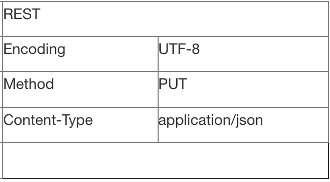
\includegraphics[scale = 1]{assets/diagrams/STPRequestParams.png}
    \caption{. Dispersion Service REST API Headers}\label{fig:STPRequestParams}
\end{figure}

The specific interface required for the request must include all the necessary banking data for a payment order to be processed \cite{stp}.\\

Any bad request should be handled accordingly in Atrato’s server, but when the request is done correctly STP can respond with the following interface:

\begin{verbatim}
    {
       result: { id: number; errorDescription?: string }; 
    }
\end{verbatim}
  
The field id can be interpreted differently depending on its length. According to STP’s documentation, any number greater tan 3 digits refers to the internal reference to the newly generated payment order; if the id is lower or equal to 3 digits, then it serves as an error code which should be consulted in STP’s errors catalog. Whenever the data received refers to an error, the field errorDescription will include additional details regarding the specific response, otherwise, it will not be included in the response.\\

This service will be consumed when the balance system's trigger succesfully generates a Bank Transfer and the dispatch is either automatically triggered or manually confirmed. The system will then proceed to generate a payment order and send it through STP. The specific processes required after STP has confirmed thar the payment order was successfully generated are described in Figure \ref{fig:stp_send_payment_order}.

\begin{figure}[H]
    \centering
    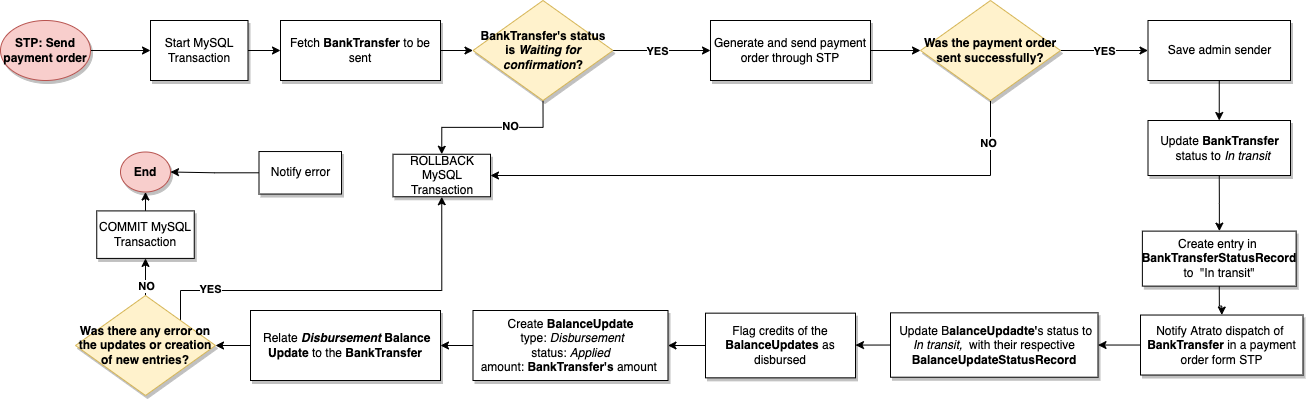
\includegraphics[scale = 0.3]{assets/flowcharts/STP_Send_Payment_Order.png}
    \caption{Balance}\label{fig:stp_send_payment_order}
\end{figure}

\section{Webhooks for Bank Transfers Status Updates}

Atrato will eventually receive an update on the status of every payment order sent through STP, which will serve as reference on how to handle the Balance Updates and Bank Transfers of every store’s balance system.\\

These status updates will be notified through a webhook that will be available through a virtual private network between Atrato’s sever and STP. Depending on the specific status updates that are received is how every balance system will execute specific logic to handle the result of every outgoing Bank Transfer.\\

Exposing this endpoint through the VPN is already a secure method for handling these status updates, nonetheless an additional security secret key generated by Atrato is required for any incoming activity. These keys will be independent for each environment.\\

\subsection{Understanding the different incoming payment order status updates}

There are only 3 different status that can be notified through this webhook: Liquidated, Cancelled or Returned.\\

Each of these different status updates will be handled independently. Whenever a payment order is Liquidated, this means that the money was correctly accepted by the receiving party. If an order is Cancelled, this means that the payment order was not even dispatched, hence, the money never left Atrato’s bank account. For the Returned status, this means that the money did leave the account, but for any external reason it had to be returned.\\

All the processes resultant of any status update will follow the same general structure and implementation as all the balance system. This means, that any error on the process will log everything on the Logs table and since everything is part of a SQL Transaction, no single object involved will be edited nor created due to the Transaction’s Rollback event. Additionally, the internal status of numerous Balance Updates and Bank Transfers will be updated; every time that this updates occur, new entries will be generated in the Balance Updates and Bank Transfers Status Record tables to keep a complete track of how each status changed over time.\\

Every Bank Transfer object generated and stored in Atrato’s database that is already sent through STP as a payment order will have the status In transit, as explained in Chapter 3. Hence, every incoming status update will trigger specific pipelines to a Bank Transfer whose current is In transit. The status to which the Bank Transfer object can changed are furtherly described in this chapter.\\

Every status update will generate an entry in the Logs table with the purpose of keeping a record of every incoming activity form STP. This will be useful for debugging any unexpected or unusual behavior in the balance system of every store.\\

The webhook exposed for these status updates works with a Switch Case architecture, with specific pipelines for every status update. Additionally, a default case as security to monitor any unexpected activity on the web service as shown in the following code snippet:\\

\begin{verbatim}
switch (statusUpdate) {
    case STPResponseStates.CANCELLED:
     await BankTransfersController.cancelSTPBankTransfer(
      bankTransfer.id
     );
     break;
 case STPResponseStates.RETURNED:
    await BankTransfersController.rejectBankTransfer(
     bankTransfer.id,
     req.body.causaDevolucion
    );
    break;
 case STPResponseStates.LIQUIDATED:
    await BankTransfersController.confirmBankTransfer(
     bankTransfer.id,
     req.body.tsLiquidacion
    );
    break;
 default:
    await STPController.notifyNotFoundStatusChange(
     req.body,
     bankTransfe?.id
    );
    break;
}

\end{verbatim}

The status of a Bank Transfer cannot deliberately change from one status to another one. There must be specific events or actions that trigger a specific change form one status to another one. These triggers are described in Figure \ref{fig:state_machine_bank_transfers}. Note how a Bank Transfer with status Waiting for confirmation can only be updated either Cancelled or to the status In transit by sending a new payment order through STP. Both states Cancelled and Rejected can be considered as final states, but the state Applied could still be furtherly updated to Rejected. Once a Bank Transfer is Applied, its state could be considered as a final state, but the rare possibility of the money being returned at some point still exists, even months after the confirmation. For this reason, there is an additional trigger that needs to be considered to update a Bank Transfer’s status from Applied to Rejected; this will be furtherly explained below.

\begin{figure}[H]
    \centering
    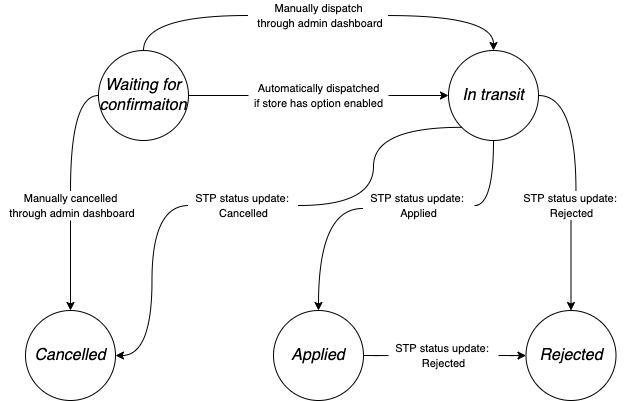
\includegraphics[scale = 0.5]{assets/diagrams/BankTransfersStateMachine.png}
    \caption{Balance Updates State Machine}\label{fig:state_machine_bank_transfers}
\end{figure}

\subsection{Liquidated status update}

This status notifies a successful bank transfer between Atrato and the receiving party. Once this status update is received the Bank Transfer object’s status related to this payment order will now be updated from In transit to Applied and all the Balance Updates that are related to this Bank Transfer will now update their status to Applied as well. Since this means that a disbursement was successfully made, a new Balance Update of type Disbursement, with status Applied, will be created to subtract to the store’s balance the amount of the Bank Transfer. Any Balance Update of type Disbursement that is created must always have their status set to Applied, so that any following Bank Transfer trigger event will not take this Balance Update into account.\\

Furthermore, the credits of which their Balance Update of type Contribution were included in this Bank Transfer can now be flagged as Disbursed. This will only serve as an indication in the merchant’s dashboard showing that these credits have already been disbursed.

\begin{figure} [h]
    \centering
    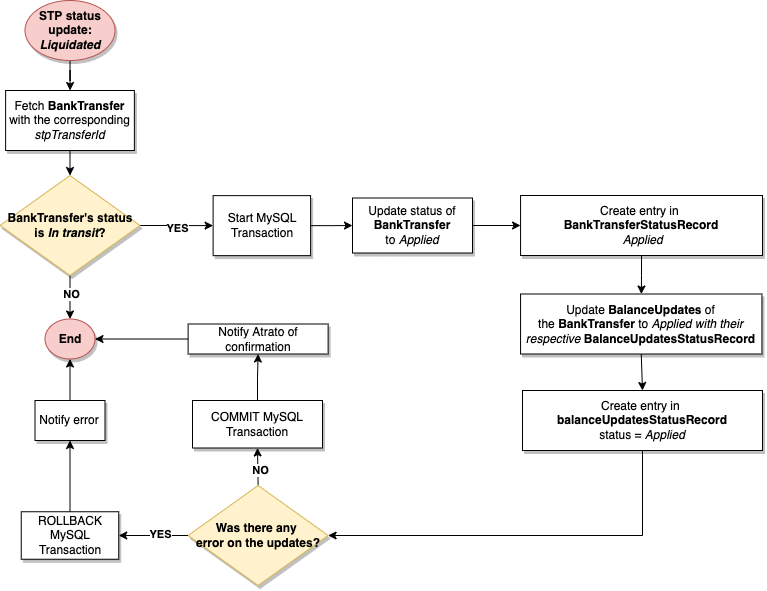
\includegraphics[scale = 0.4]{assets/diagrams/LiquidatedStatusUpdate.png}
    \caption{Processing internal status of Balance Updates and Bank Transfer for Liquidated payment orders}\label{fig:liquidated_status_update}
\end{figure}

\subsection{Cancelled status update}

This status does not happen very often, but still needs to be considered. Whenever a Bank Transfer is cancelled its status will be updated to Cancelled and no further action will be taken regarding a cancelled Bank Transfer, since this is a final state. In terms of the Balance Updates that composed this Bank Transfer, their status will be updated back to Pending, meaning that they could and will be considered for the next Bank Transfer generated once the Bank Transfer’s trigger takes place.\\

This does not necessarily mean that a new Bank Transfer object with the same amount and same related Balance Update objects will be generated because it will depend entirely on the next bank transfer generation event that is triggered and the Balance Updates that have a status of pending by the time the trigger takes place.

\begin{figure} [h]
    \centering
    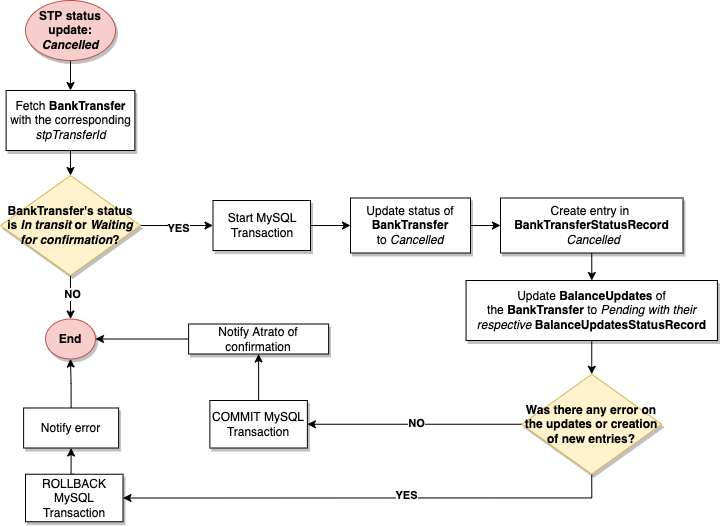
\includegraphics[scale = 0.4]{assets/diagrams/CancelledStatusUpdate.png}
    \caption{Processing internal status of Balance Updates and Bank Transfer for Cancelled payment orders}\label{fig:cancelled_status_update}
\end{figure}

\subsection{Returned status update}

If a payment order is returned, the process that the Bank Transfer object will follow depends on its state. If the state is In transit, meaning it is a Bank Transfer that was recently sent through a payment order, then the Bank Transfer object related to this order will update its status to Rejected and the process regarding to the Balance Updates will be very similar to a cancellation: their status will be updated back to Pending so that they can be considered in a new Bank Transfer in the next trigger. Since no additional updates were made to the store’s general balance then no further action is required, just as in a cancellation.\\

Meanwhile, if the status of the Bank Transfer object is already Applied, then additional to the previous process of updating the Balance Updates back to Pending, further actions need to be taken. Moneywise, the Balance Updates that were previously confirmed, but now the money was returned to Atrato’s account, meaning that they should be considered in a new Bank Transfer.\\

For this specific scenario, a new Balance Update of type Disbursement was already generated when the Bank Transfer was previously confirmed, so a new Balance Update of type Disbursement Override needs to be generated to compensate the changes made to the store’s balance. This new Balance Update will directly update the store’s balance; hence, it will automatically have the status of Applied.\\

By updating the previously confirmed Balance Updates back to Pending, they will eventually be considered into a new Bank Transfer.

\begin{figure} [h]
    \centering
    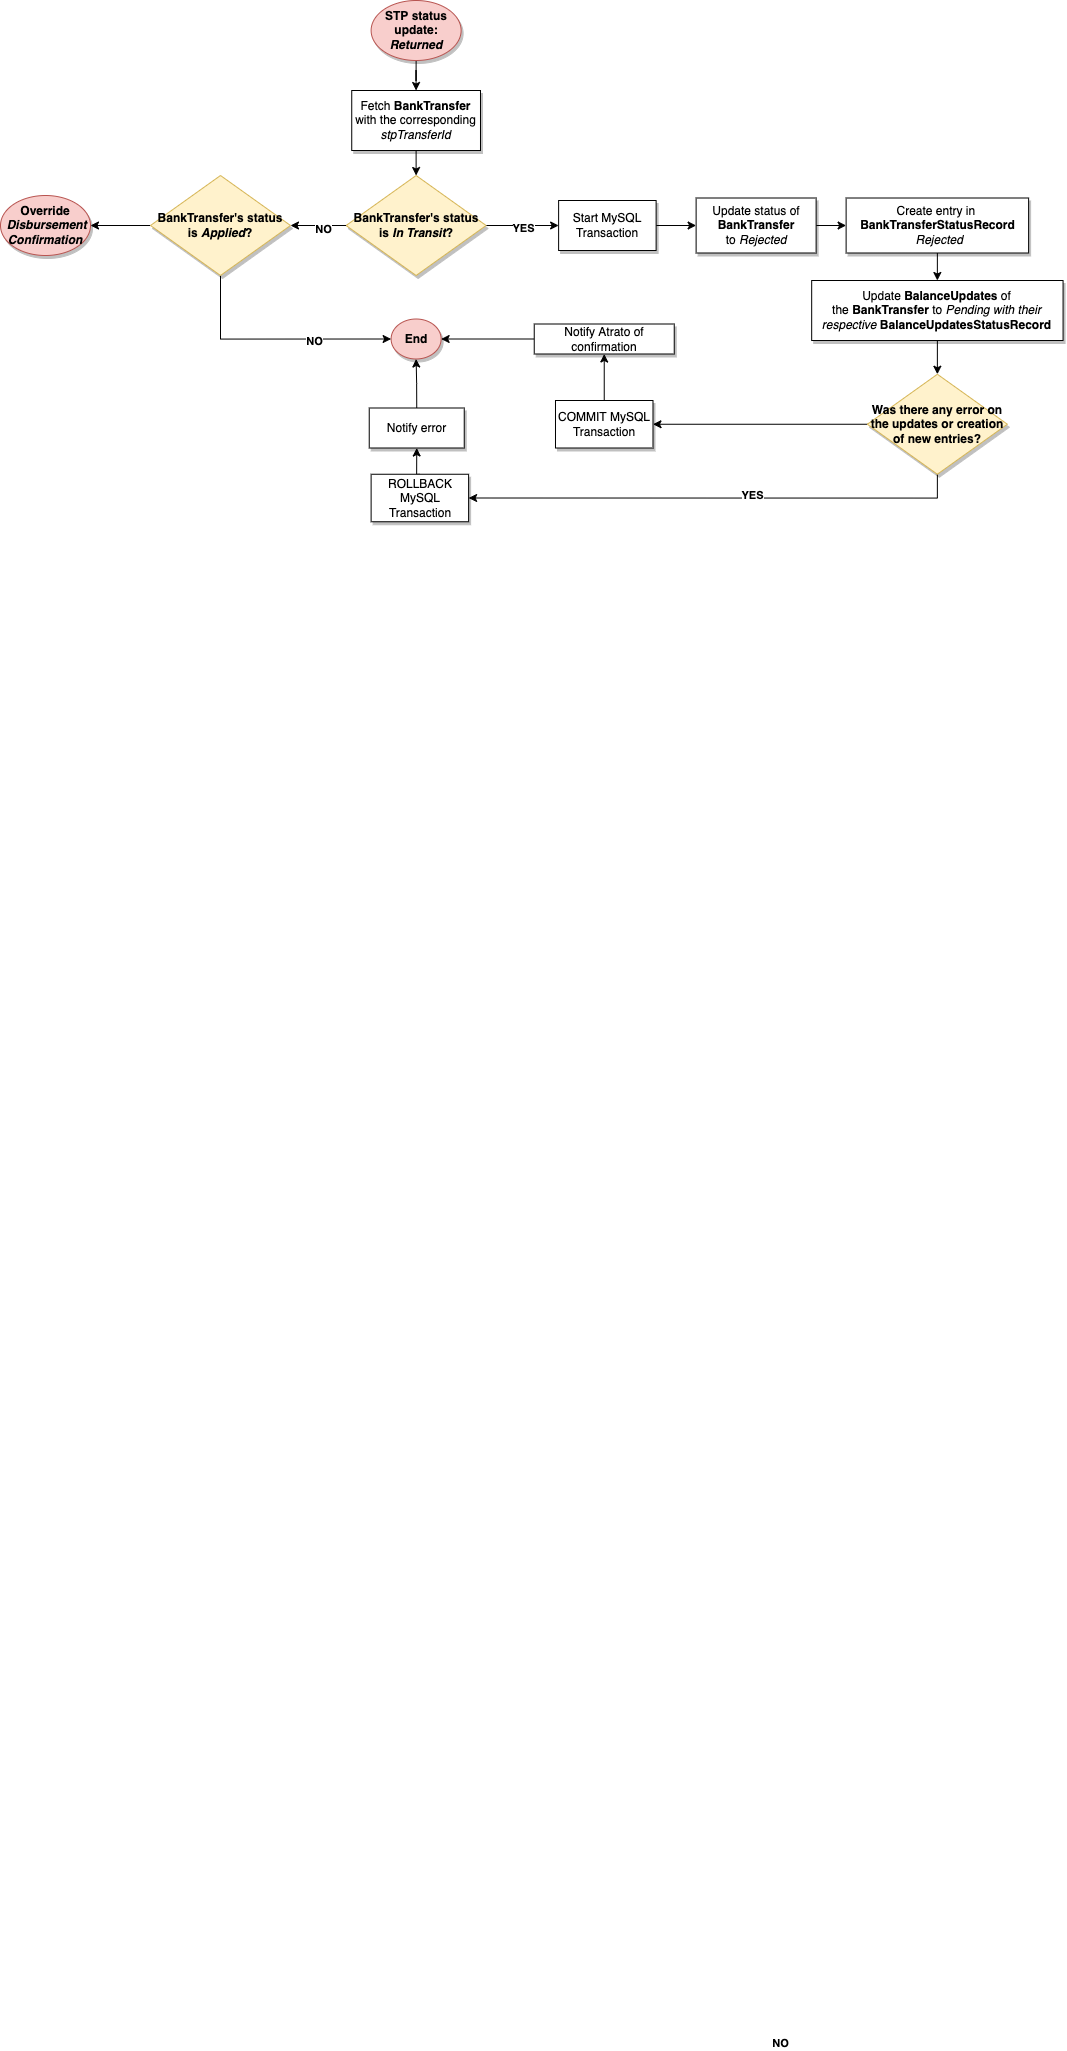
\includegraphics[scale = 0.4]{assets/diagrams/ReturnedStatusUpdate.png}
    \caption{Processing internal status of Balance Updates and Bank Transfer for Returned payment orders. Note the similarity with the Cancelation process}\label{fig:returned_status_update}
\end{figure}
